\chapter{EQUIPMENT}

\begin{multicols}{2}

\index{Equipment}While each class offers its own unique talents and abilities, a character is nothing without equipment.  Equipment comes in the form of armor to protect him, weapons to strike down his enemies, food to keep him fed, blankets to keep him warm, and the money he uses to purchase it.  This section isn't a detailed description of in-game economy although a working system can be built using it.

\index{Coins}There are five primary currencies, based on the metal they're minted from. They are assumed to be in universal use across the world.  The names are generic and the exchange rates fixed, however, this is merely the information given to the player characters.  It's up to the GM to decide if he should change, rename, or even drop currency altogether.  Copper and silver coins minted in one realm and the corresponding coins of a neighboring realm may be worth drastically different rates, especially when the currency crosses the border.  Generally speaking, though, the price of gold is the same across the world.

The basic coins of the realm are the copper piece (cp) and silver piece (sp).  These are the coins used by ``common folk" in day-to-day exchanges.  More rare is the gold piece (gp), which is used by big businesses such as banks, ranking authority, and adventurers.  The gp is the standardized coin for adventurers and most prices are based on it.  The most rare coins are the electrum piece (ep) and platinum piece (pp).  These coins are no longer being minted, are of dubious value in the open market, and are only found among ancient treasure troves and amongst collectors.  That's not to say a shop won't take them, however, a shopkeeper is more willing to accept a standardized and currently minted gold coin than an ep or pp.

There are other means of exchange and very rarely do the common folk deal with coins alone.  Coins depreciate in value, whereas objects don't.  Coins aren't very portable in large amounts, whereas objects can be worth thousands while maintaining a fraction of the weight.  A flawless emerald, the deed to land, and even a pig or cow make excellent forms of portable wealth and most people are more than willing to trade for them.

\noindent
\begin{minipage}{\columnwidth}

\captionof{table}{Exchange Rates}\label{exchangerates}
\noindent
\begin{tabular}{|p{0.2\columnwidth}|p{0.1\columnwidth}|p{0.1\columnwidth}|p{0.1\columnwidth}|p{0.1\columnwidth}|p{0.1\columnwidth}|}
\hline
Coin	& CP	& SP	& EP	& GP	& PP \\
\hline\hline
\rowcolor[gray]{.9}Copper Piece (CP)	& 1	& 1/10	& 1/50	& 1/100	& 1/500 \\
Silver Piece (SP)	& 10	& 1	& 1/5	& 1/10	& 1/50 \\
\rowcolor[gray]{.9}Electrum Piece (EP)	& 50	& 5	& 1	& 1/5	& 1/10 \\
Gold Piece (GP)		& 100	& 10	& 2	& 1	& 1/5 \\
\rowcolor[gray]{.9}Platinum Piece (PP)	& 500	& 50	& 10	& 5	& 1 \\
\hline
\end{tabular}

\end{minipage}

All coins, regardless of metal, weigh 1 pound per 50 units.  Metal bars also make good, portable currency.  A 1-pound bar of gold, for example, is always worth 50 gp.

\section{STARTING MONEY}

\index{Starting Money}All starting PCs begin with a certain amount of money.  This may reflect a sudden windfall, the character's life savings, gifts from family, or any aspect that would make sense within the game world.  Starting funds should never be shared or lent during character creation even if the characters are family, friends, or acquaintances.  Starting funds are based on class, and multi-class characters pick the most advantageous row.  The number in parenthesis is the average value.

\noindent
\begin{minipage}{\columnwidth}

\captionof{table}{PC Starting Money}\label{exchangerates}
\noindent
\begin{tabular}{|p{0.24\columnwidth}|p{0.66\columnwidth}|}
\hline
Class	& Starting Funds \\
\hline\hline
\rowcolor[gray]{.9}Warrior	& 5d4~$\times$~10 gp (100 gp) \\
Wizard	& (1d4~+~1)~$\times$~10 gp (30 gp) \\
\rowcolor[gray]{.9}Rogue	& 2d6~$\times$~10 gp (60 gp) \\
Priest*	& 3d6~$\times$~10 gp (90 gp) \\
\hline
\end{tabular}
\noindent\begin{tabular}{p{.95\columnwidth}}
*After purchasing their equipment, priests are allowed to keep 1d3 gold pieces.  The rest must be donated to their organization or church. \\
\end{tabular}\vspace{.5em}

\end{minipage}

\section{STANDARD EQUIPMENT LISTS}

The equipment lists show the average value of many items a starting character would commonly have access to.  The lists do not reflect the current state of the economy, supply, or demand.  The prices are guidelines, and they can fluctuate higher or be haggled down to better deals.  The more unusual items include descriptions.

\noindent
\begin{minipage}{\columnwidth}

\captionof{table}{Carrying Capacity}\label{capacity}
\noindent
\begin{tabular}{|p{0.28\columnwidth}|p{0.28\columnwidth}|p{0.29\columnwidth}|}
\hline
Item	& Capacity	& Volume \\
\hline\hline
\rowcolor[gray]{.9}Backpack	& 50 lbs.	& 3'~$\times$~2'~$\times$~1' \\
Basket	& 	& \\
\hspace{1em}Large	& 20 lbs.	& 2'~$\times$~2'~$\times$~2' \\
\rowcolor[gray]{.9}\hspace{1em}Small	& 10 lbs.	& 1'~$\times$~1'~$\times$~1' \\
Belt Pouch	& 	& \\
\hspace{1em}Large	& 8 lbs.	& 6"~$\times$~8"~$\times$~2" \\
\rowcolor[gray]{.9}\hspace{1em}Small	& 5 lbs.	& 4"~$\times$~6"~$\times$~2" \\
Chest	& 	& \\
\hspace{1em}Large	& 100 lbs.	& 3'~$\times$~2'~$\times$~2' \\
\rowcolor[gray]{.9}\hspace{1em}Small	& 40 lbs.		& 2'~$\times$~1'~$\times$~1' \\
Sack	& 	& \\
\hspace{1em}Extra-large*	& 80 lbs.	& 4'~$\times$~2'~$\times$~2' \\
\rowcolor[gray]{.9}\hspace{1em}Large	& 30 lbs.	& 2'~$\times$~2'~$\times$~1' \\
\hspace{1em}Small	& 15 lbs.	& 1'~$\times$~1'~$\times$~8" \\
\rowcolor[gray]{.9}\hspace{1em}Tiny	& 4 lbs.	& 6"~$\times$~6"~$\times$~4" \\
Saddle Bags	& 	& \\
\hspace{1em}Large	& 30 lbs.	& 18"~$\times$~1'~$\times$~6" \\
\rowcolor[gray]{.9}\hspace{1em}Small	& 20 lbs.	& 1'~$\times$~1'~$\times$~6" \\
\hline
\end{tabular}
\noindent\begin{tabular}{p{.95\columnwidth}}
*When filled, these sacks are medium-sized. \\
\end{tabular}\vspace{.5em}

\end{minipage}

\noindent
\begin{minipage}{\columnwidth}

\index{Clothing}\captionof{table}{Clothing}\label{clothing}
\noindent
\begin{tabular}{|p{0.72\columnwidth}|p{0.18\columnwidth}|}
\hline
Item	& Cost \\
\hline\hline
\rowcolor[gray]{.9}Belt	& 3 sp \\
Boots & \\
\hspace{1em}Riding	& 3 gp \\
\rowcolor[gray]{.9}\hspace{1em}Soft	& 1 gp \\
Breeches	& 2 gp \\
\rowcolor[gray]{.9}Cap, hat	& 1 sp \\
Cloak & \\
\hspace{1em}Good cloth	& 8 sp \\
\rowcolor[gray]{.9}\hspace{1em}Common fur	& 50 gp \\
Girdle	& 3 gp \\
\rowcolor[gray]{.9}Gloves	& 1 gp \\
Gown, common	& 12 sp \\
\rowcolor[gray]{.9}Hose	& 2 gp \\
Knife sheath	& 3 cp \\
\rowcolor[gray]{.9}Mittens	& 3 sp \\
Pin	& 6 gp \\
\rowcolor[gray]{.9}Plain brooch	& 10 gp \\
Robe	& \\
\hspace{1em}Common	& 9 sp \\
\rowcolor[gray]{.9}\hspace{1em}Embroidered	& 20 gp \\
Sandals	& 5 cp \\
\rowcolor[gray]{.9}Sash	& 2 sp \\
Shoes	& 1 gp \\
\rowcolor[gray]{.9}Silk jacket	& 80 gp \\
Surcoat	& 6 sp \\
\rowcolor[gray]{.9}Sword scabbard, hanger, baldric	& 4 gp \\
Tabard	& 6 sp \\
\rowcolor[gray]{.9}Toga, coarse	& 8 cp \\
Tunic	& 8 sp \\
\rowcolor[gray]{.9}Vest	& 6 sp \\
\hline
\end{tabular}

\end{minipage}

\noindent
\begin{minipage}{\columnwidth}

\captionof{table}{Miscellaneous Equipment}\label{miscequip}
\noindent
\begin{tabular}{|p{0.55\columnwidth}|p{0.16\columnwidth}|p{0.14\columnwidth}|}
\hline
Item	& Cost	& Weight (in lbs.)\\
\hline\hline
\rowcolor[gray]{.9}Backpack		& 2 gp	& 2 \\
Barrel, Small	& 2 gp	& 30 \\
\rowcolor[gray]{.9}Basket			& 	& \\
\rowcolor[gray]{.9}\hspace{1em}Large			& 3 sp	& 1 \\
\hspace{1em}Small			& 5 cp	& .01 \\
\rowcolor[gray]{.9}Bell			& 1 gp	& -- \\
Belt pouch		& 	& \\
\hspace{1em}Large			& 1 gp	& 1 \\
\rowcolor[gray]{.9}\hspace{1em}Small			& 7 sp	& 0.5 \\
Block and tackle	& 5 gp	& 5 \\
\rowcolor[gray]{.9}Bolt case		& 1 gp	& 1 \\
Bucket			& 5 sp	& 3 \\
\rowcolor[gray]{.9}Chain (per foot)	& 	& \\
\rowcolor[gray]{.9}\hspace{1em}Heavy			& 4 gp	& 3 \\
\hspace{1em}Light			& 3 gp	& 1 \\
\rowcolor[gray]{.9}Chest			& 	& \\
\rowcolor[gray]{.9}\hspace{1em}Large			& 2 gp	& 25 \\
\hspace{1em}Small			& 1 gp	& 10 \\
\rowcolor[gray]{.9}Cloth (per 10 square yards)	& 	& \\
\rowcolor[gray]{.9}\hspace{1em}Common		& 7 gp	& 10 \\
\hspace{1em}Fine			& 50 gp	& 10 \\
\rowcolor[gray]{.9}\hspace{1em}Rich			& 100 gp	& 10 \\
Candle, tallow	& 1 cp	& 0.1 \\
\rowcolor[gray]{.9}Candle, wax		& 1 sp	& 0.1 \\
Canvas (per square yard)	& 4 sp	& 1 \\
\rowcolor[gray]{.9}Chalk			& 1 cp	& 0.1 \\
Crampons			& 4 gp	& 2 \\
\rowcolor[gray]{.9}Fishhook			& 1 sp	& .01 \\
Fishing net, 10 feet square	& 4 gp	& 5 \\
\rowcolor[gray]{.9}Flint and steel		& 5 sp	& 0.1 \\
Glass bottle		& 10 gp	& 0.1 \\
\hline
\end{tabular}
\noindent
\begin{tabular}[r]{p{.95\columnwidth}}
\textit{continued on next column \ldots} \\
\end{tabular}

\end{minipage}

\noindent
\begin{minipage}{\columnwidth}

\noindent
\begin{tabular}[c]{p{.95\columnwidth}}
\textit{\ldots continued from previous column} \\
\end{tabular}

\noindent
\begin{tabular}{|p{0.55\columnwidth}|p{0.16\columnwidth}|p{0.14\columnwidth}|}
\hline
Item	& Cost	& Weight (in lbs.)\\
\hline\hline
\rowcolor[gray]{.9}Grappling hook		& 8 sp	& 4 \\
Holy item 			& 25 gp	& 0.1 \\
\rowcolor[gray]{.9}Hourglass			& 25 gp	& 1 \\
Iron pot			& 5 sp	& 2 \\
\rowcolor[gray]{.9}Ladder, 10 feet		& 5 cp	& 20 \\
Lantern				& 	& \\
\hspace{1em}Beacon			& 150 gp	& 50 \\
\rowcolor[gray]{.9}\hspace{1em}Bull's-eye		& 12 gp	& 3 \\
\hspace{1em}Hooded			& 7 gp	& 2 \\
\rowcolor[gray]{.9}Lock				& 	& \\
\rowcolor[gray]{.9}\hspace{1em}Good				& 100 gp	& 1 \\
\hspace{1em}Poor				& 20 gp	& 1 \\
\rowcolor[gray]{.9}Magnifying Glass	& 100 gp	& 0.1 \\
Map or scroll case 	& 8 sp	& 0.5 \\
\rowcolor[gray]{.9}Merchant's scale	& 2 gp	& 1 \\
Mirror, small metal	& 10 gp	& 0.1 \\
\rowcolor[gray]{.9}Musical instrument	& 5--100 gp	& 0.5--3 \\
Oil (per flask)		& 	& \\
\hspace{1em}Greek fire		& 10 gp	& 2 \\
\rowcolor[gray]{.9}\hspace{1em}Lamp				& 6 cp	& 1 \\
Paper (per sheet)	& 2 gp	& 0.01 \\
\rowcolor[gray]{.9}Papyrus (per sheet)	& 8 sp	& 0.01 \\
Parchment (per sheet)	& 1 gp	& 0.01 \\
\rowcolor[gray]{.9}Perfume (per vial)	& 5 gp	& 0.1 \\
Piton				& 3 cp	& 0.5 \\
\rowcolor[gray]{.9}Quiver				& 8 sp	& 1 \\
Rope (per 50 feet)	& 	& \\
\hspace{1em}Hemp				& 1 gp	& 20 \\
\rowcolor[gray]{.9}\hspace{1em}Silk				& 10 gp	& 8 \\
Sack				& 	& \\
\hspace{1em}Extra-large		& 7 sp	& 1 \\
\rowcolor[gray]{.9}\hspace{1em}Large				& 2 sp	& 0.5 \\
\hspace{1em}Small				& 5 cp	& 0.1 \\
\rowcolor[gray]{.9}\hspace{1em}Tiny				& 2 cp	& 0.01 \\
Sealing/candle wax (per lb.)	& 1 gp	& 1 \\
\rowcolor[gray]{.9}Sewing needle		& 5 sp	& 0.01 \\
Signal whistle		& 8 sp	& 0.1 \\
\rowcolor[gray]{.9}Signet ring or personal seal	& 5 gp	& 0.1 \\
Soap (per lb.)		& 5 sp	& 1 \\
\rowcolor[gray]{.9}Spyglass			& 1,000 gp	& 1 \\
Tent				& 	& \\
\hspace{1em}Large				& 25 gp	& 20 \\
\rowcolor[gray]{.9}\hspace{1em}Pavilion			& 100 gp	& 50 \\
\hspace{1em}Small				& 5 gp	& 10 \\
\rowcolor[gray]{.9}Thieves' picks		& 30 gp	& 1 \\
Torch				& 1 cp	& 1 \\
\rowcolor[gray]{.9}Water clock			& 1,000 gp	& 200 \\
Whetstone			& 2 cp	& 1 \\
\rowcolor[gray]{.9}Wineskin			& 8 sp	& 1 \\
Winter blanket		& 5 sp	& 3 \\
\rowcolor[gray]{.9}Writing ink (per vial)	& 8 gp	& 0.1 \\
\hline
\end{tabular}

\end{minipage}

\index{Holy Items}\paragraph{Holy Item:} Symbols and blessed items revered by a religious organization.  Holy items can include holy water, a symbol like the cross, mistletoe (for druids), sacred scripture, wine, oils, precious metals, etc.  What counts as a holy item is up to the faith itself.  Holy items by themselves are powerless but when blessed by a priest of the faith in a special ceremony they can be used as a component for spells or harming undead.  Any rule that refers to a holy symbol or water applies to all holy items so long as they are blessed or specially prepared.

Holy items usually cannot be purchased.  A priest of the faith can requisition them but religious organizations are protective of their blessed items for fear of being used against their intended purpose.  Non-priests of the faith can requisition holy items only if the need is pressing.

\index{Lanterns}\paragraph{Lanterns:} A hooded lantern has a shutter to dim light and can project light in a 30-foot radius.  Bull's-eye lanterns have a single shutter that project a cone-shaped beam of light, 60-foot cone long and 20 feet wide.  Beacon lanterns are unfit for personal carrying and they're usually mounted to buildings, ships, and wagons.  Beacon lanterns project a cone-shaped beam of light, 240-foot cone long and 90 feet wide.  Hooded and bull's-eye lanterns burn one flask (one pint) of oil every 6 hours.  Beacon lanterns require a flask of oil every 2 hours.

\noindent
\includegraphics[width=\columnwidth, height=4in]{testblock.pdf} 

\index{Locks}\paragraph{Locks:}  Locks are large, bulky devices that work with a single key.  Combination locks are relatively unheard of.  The quality of a lock determines how difficult it is to pick or destroy.

Poor and good locks are commonly found in stores.  Higher quality locks can be built at an increased price.  Locks of poorer quality are usually second hand or decrepit because of age.  The quality of the lock can increase or decrease the chance to pick it.  A thief usually cannot tell the quality of a lock simply by study, only by attempting to pick it.

\noindent
\begin{minipage}{\columnwidth}

\captionof{table}{Lock Quality Modifiers}\label{lockqual}
\noindent
\begin{tabular}{|p{0.45\columnwidth}|p{0.45\columnwidth}|}
\hline
Quality		& Modification \\
\hline\hline
\rowcolor[gray]{.9}Wretched	& +30\% \\
Poor		& +15\% \\
\rowcolor[gray]{.9}Good		& 0\% \\
Excellent	& $-20$\% \\
\rowcolor[gray]{.9}Superior	& $-40$\% \\
Masterful	& $-60$\% \\
\hline
\end{tabular}

\end{minipage}

\index{Magnifying Glasses}\paragraph{Magnifying Glass:} A circular prism about 6 inches in diameter and set in a frame with a handle usually made of wood or metal.  It is a novelty more than a true tool.  The technology to craft good ones doesn't exist, making the lens distort and the magnification poor.  Useful for starting fires on a sunny, clear day.

\index{Merchant's Scales}\paragraph{Merchant's Scale:}  A small balance and pans with appropriately sized lead weights.  Merchant's scales are used to measure the weight of coins during transactions.  Scales can be rigged using hollow or heavier weights to cheat unsuspecting victims.  Some civilizations may mandate annual calibration tests.  

\index{Oil}\paragraph{Oil:}  Greek fire uses a sticky, tar-like flammable substance and is thrown at opponents.  Lamp oil is generally used to fill lamps but can also be made into a flammable weapon.

\index{Quivers}\paragraph{Quiver:} Quivers come in hip, back, ground, and bow.  Hip and back quivers are medium size and hold 24 arrows or bolts.  Bow quivers attach directly to the bow or crossbow and hold 6 arrows or bolts.  Ground quivers are simple metal poles or racks that jut out the ground and can hold 2 bows or crossbows and 48 arrows or bolts.  Because of their limited portability, ground quivers are used during war when archers need ready access to massive amounts of ammunition.

\index{Spyglasses}\paragraph{Spyglass:}  More of a novelty than a useful tool.  Only provides about three times magnification and objects are usually distorted.

\noindent
\begin{minipage}{\columnwidth}

\index{Provisions}\captionof{table}{Provisions}\label{provisions}
\noindent
\begin{tabular}{|p{0.72\columnwidth}|p{0.18\columnwidth}|}
\hline
Item					& Cost \\
\hline\hline
\rowcolor[gray]{.9}Barrel of picked fish	& 3 gp \\
Butter (per lb.)		& 2 sp \\
\rowcolor[gray]{.9}Coarse sugar (per lb.)	& 1 gp \\
Dry rations (per week)	& 10 gp \\
\rowcolor[gray]{.9}Eggs (per 100)/ per two dozen	& 8 sp, 2 sp \\
Figs (per lb.)			& 3 sp \\
\rowcolor[gray]{.9}Firewood (per day)		& 1 cp \\
Herbs (per day)			& 5 cp \\
\rowcolor[gray]{.9}Nuts (per lb.)			& 1 gp \\
Raisins (per lb.)		& 2 sp \\
\rowcolor[gray]{.9}Rice (per lb.)			& 2 sp \\
Salt (per lb.)			& 1 sp \\
\rowcolor[gray]{.9}Salted herring (per 100)	& 1 gp \\
Spice, Exotic (saffron, clove, cumin) (per lb.)	& 15 gp \\
\rowcolor[gray]{.9}Spice, Rare (pepper, ginger, basil) (per lb.)	& 2 gp \\
Spice, Uncommon (cinnamon, nutmeg) (per lb.)	& 1 gp \\
\rowcolor[gray]{.9}Tun of cider (250 gal.)	& 8 gp \\
Tun of good wine (250 gal.)	& 20 gp \\
\hline
\end{tabular}

\end{minipage}

\index{Thieves' Picks}\paragraph{Thieves' Picks:} A collection of metal rods, picks, a clamp, wedge, hammer, and a saw.  Allows a thief to pick locks and remove traps without penalty.  

\index{Water Clocks}\paragraph{Water Clock:} Measures time by dripping water into a basin that moves a rod and subsequently calculates the time.  Accurate up to a half-hour, they are large, expensive, and clunky devices, usually owned by the wealthy.

\noindent
\begin{minipage}{\columnwidth}

\captionof{table}{Provisions}\label{provisions}
\noindent
\begin{tabular}{|p{0.72\columnwidth}|p{0.18\columnwidth}|}
\hline
Item				& Cost \\
\hline\hline
\rowcolor[gray]{.9}Ale (per gallon)		& 2 sp \\
Banquet (per person)	& 10 gp \\
\rowcolor[gray]{.9}Bread					& 5 cp \\
Cheese					& 4 sp \\
\rowcolor[gray]{.9}City rooms, Common (per month)		& 20 gp \\
City rooms, Poor (per month)		& 6 sp \\
\rowcolor[gray]{.9}Common wine (pitcher)				& 2 sp \\
Eggs or fresh vegetables			& 1 cp \\
\rowcolor[gray]{.9}Honey					& 5 sp \\
Inn lodging, Common (per day/week)	& 5 sp/3 gp \\
\rowcolor[gray]{.9}Inn lodging, Common (per day/week)	& 5 cp/2 sp \\
Meat (one meal)			& 1 sp \\
\rowcolor[gray]{.9}Meals, Good (per day)	& 5 sp \\
Meals, Common (per day)	& 3 sp \\
\rowcolor[gray]{.9}Meals, Poor (per day)	& 1 sp \\
Separate latrine for rooms (per month)	& 2 gp \\
\rowcolor[gray]{.9}Small beer (per gallon)	& 5 cp \\
Soup					& 5 cp \\
\hline
\end{tabular}

\end{minipage}

\noindent
\begin{minipage}{\columnwidth}

\captionof{table}{Living Conditions}\label{livingconditions}
\noindent
\begin{tabular}{|p{0.6\columnwidth}|p{0.3\columnwidth}|}
\hline
Lifestyle	& Cost/Month \\
\hline\hline
\rowcolor[gray]{.9}Squalid		& 3 gp \\
Poor		& 5 gp \\
\rowcolor[gray]{.9}Middle-Class	& 50 gp/level \\
Wealthy		& 200 gp/level \\
\hline
\end{tabular}

\end{minipage}

\noindent
\begin{minipage}{\columnwidth}

\index{Services}\captionof{table}{Services}\label{livingconditions}
\noindent
\begin{tabular}{|p{0.72\columnwidth}|p{0.18\columnwidth}|}
\hline
Service						& Cost \\
\hline\hline
\rowcolor[gray]{.9}Bath						& 3 cp \\
Clerk (per letter)			& 2 sp \\
\rowcolor[gray]{.9}Doctor, leech, or bleeding	& 3 gp \\
Guide, city (per day)		& 2 sp \\
\rowcolor[gray]{.9}Lantern or torchbearer (per night)	& 1 sp \\
Laundry (by load)			& 1 cp \\
\rowcolor[gray]{.9}Messenger, city (per message)	& 1 sp \\
Minstrel (per performance)	& 3 gp \\
\rowcolor[gray]{.9}Mourner (per funeral)		& 2 sp \\
Teamster w/wagon			& 1 sp/mile \\
\hline
\end{tabular}

\end{minipage}

\noindent
\begin{minipage}{\columnwidth}

\captionof{table}{Animals}\label{animals}
\noindent
\begin{tabular}{|p{0.72\columnwidth}|p{0.18\columnwidth}|}
\hline
Item				& Cost \\
\hline\hline
\rowcolor[gray]{.9}Boar				& 10 gp \\
Bull				& 20 gp \\
\rowcolor[gray]{.9}Calf				& 5 gp \\
Camel				& 50 gp \\
\rowcolor[gray]{.9}Capon				& 3 cp \\
Cat					& 1 sp \\
\rowcolor[gray]{.9}Chicken				& 2 cp \\
Cow					& 10 gp \\
\rowcolor[gray]{.9}Dog					&  \\
\rowcolor[gray]{.9}\hspace{1em}Guard				& 25 gp \\
\hspace{1em}Hunting			& 17 gp \\
\rowcolor[gray]{.9}\hspace{1em}War				& 20 gp \\
Donkey, mule, ass	& 8 gp \\
\rowcolor[gray]{.9}Elephant			&  \\
\rowcolor[gray]{.9}\hspace{1em}Labor				& 200 gp \\
\hspace{1em}War				& 500 gp \\
\rowcolor[gray]{.9}Falcon (trained)	& 1,000 gp \\
Goat				& 1 gp \\
\rowcolor[gray]{.9}Goose				& 5 cp \\
Guinea Hen			& 2 cp \\
\rowcolor[gray]{.9}Horse				&  \\
\rowcolor[gray]{.9}\hspace{1em}Draft				& 200 gp \\
\hspace{1em}Heavy war			& 400 gp \\
\rowcolor[gray]{.9}\hspace{1em}Light war			& 150 gp \\
\hspace{1em}Medium war		& 225 gp \\
\rowcolor[gray]{.9}\hspace{1em}Riding			& 75 gp \\
Hunting cat (jaguar, panther, etc.)	& 5,000 gp \\
\rowcolor[gray]{.9}Ox					& 15 gp \\
Partridge			& 5 cp \\
\rowcolor[gray]{.9}Peacock				& 5 sp \\
Pig					& 3 gp \\
\rowcolor[gray]{.9}Pigeon				& 1 cp \\
Pigeon, messenger	& 100 gp \\
\rowcolor[gray]{.9}Pony				& 30 gp \\
Ram					& 4 gp \\
\rowcolor[gray]{.9}Sheep				& 2 gp \\
Songbird			& 10 sp \\
\rowcolor[gray]{.9}Swan				& 5 sp \\
\hline
\end{tabular}

\end{minipage}

\noindent
\includegraphics[width=\columnwidth, height=2.5in]{testblock.pdf} 

\noindent
\includegraphics[width=\columnwidth, height=2in]{testblock.pdf} 

\index{Animals}\index{Horses}\paragraph{Horses:} Horses require adequate forage to eat or a bag of good quality grain each day.  Heavy warhorses cannot survive on grazing alone and all horses require water each day.  At night, horses must be tethered on a long strand so they can forage and their saddles or packs must be removed.

The common horse is of average quality with no unique quirks or flaws.  Horses of various qualities can be introduced which may decrease or increase the price.  Unscrupulous merchants can try to pawn off poor quality horses as average.

\noindent
\begin{minipage}{\columnwidth}

\captionof{table}{Horse Quality}\label{horsequality}
\noindent
\begin{tabular}{|p{0.26\columnwidth}|p{0.18\columnwidth}|p{0.18\columnwidth}|p{0.18\columnwidth}|}
\hline
Quality	& Movement Rate Modifier	& Carrying Capacity Modifier	& Cost Modifier \\
\hline\hline
\rowcolor[gray]{.9}Nag				& 50\%	& 25\%	& -- \\
Broken-down		& 75\%	& 50\%	& -- \\
\rowcolor[gray]{.9}Average			& --	& --	& -- \\
High-spirited	& 133\%	& 125\%	& $\times$2 \\
\rowcolor[gray]{.9}Charger			& 150\%	& 133\%	& $\times$4 \\
\hline
\end{tabular}

\end{minipage}

\index{Pony}\index{Donkey}\index{Mule}\paragraph{Ponies, donkeys, and mules:} Hardier than horses, they require adequate food and water each day but can survive on grass and other forage alone.  They gain a +2 bonus on their save vs. death when double moving (but not triple moving).  They can travel through rugged terrain at one less the normal movement value.  Ponies, donkeys, and mules don't wander off like horses thus they don't need to be tethered.

\index{Camel}\paragraph{Camels:} Camels come in two types; Dromedary (sandy desert) and Bactrian (rocky desert).  Dromedaries reduce the movement value in sandy deserts by 1 point.  Bactrians reduce the movement value in rocky deserts by 1 point.  Camels can survive on grazing and must have adequate food each day and water every four days (longer if green food is available).  Camels must be tethered or they wander off.

\index{Dog}\paragraph{Dogs:} Some dogs are trained for carrying small riders, but many more are used to pull sleds by man-sized creatures.  Dogs require water and at least a pound of meat each day.  Dogs are gregarious and thus never wander far from their owner.

\index{Elephant}\paragraph{Elephants:} In thickly forested areas, an elephant has enough food to satisfy its hunger.  In sparsely vegetated areas it can only move at $^1$/$_4$ its normal movement value each day; the rest must be spent eating.  Elephants cannot navigate cliffs with steep slopes.  If it tries to go down a steep decline it must make a save vs. breath weapon or lose footing and tumble to the bottom.  Elephants are unaffected by mud.  Elephants don't wander far and don't need to be tethered.

\index{Yak}\paragraph{Yaks:} Yaks are suited for cold regions.  They reduce the penalty to movement value for mountains by one.  They can survive on small amounts of grass and water each day and can provide milk to travelers.  Yaks cannot survive in warmer climates, as they're prone to heat exhaustion. 

\columnbreak

\noindent
\begin{minipage}{\columnwidth}

\captionof{table}{Tack and Harness}\label{tackharness}
\noindent
\begin{tabular}{|m{0.57\columnwidth}|m{0.13\columnwidth}|m{0.15\columnwidth}|}
\hline
Item	& Cost	& Weight (in lbs.) \\
\hline\hline
\rowcolor[gray]{.9}Barding			& 	&  \\
\rowcolor[gray]{.9}\hspace{1em}Chain			& 500 gp	& 70 \\
\hspace{1em}Full plate	& 2,000 gp	& 85 \\
\rowcolor[gray]{.9}\hspace{1em}Full scale	& 1,000 gp	& 75 \\
\hspace{1em}Half brigandine	& 500 gp	& 45 \\
\rowcolor[gray]{.9}\hspace{1em}Half padded	& 100 gp	& 25 \\
\hspace{1em}Half scale	& 500 gp	& 50 \\
\rowcolor[gray]{.9}\hspace{1em}Leather or padded	& 150 gp	& 60 \\
Bit and bridle	& 15 sp	& 3 \\
\rowcolor[gray]{.9}Cart harness	& 2 gp	& 10 \\
Halter			& 5 cp	& 0.1 \\
\rowcolor[gray]{.9}Horseshoes \& shoeing	& 1 gp	& 10 \\
Saddle			& 	&  \\
\hspace{1em}Pack			& 5 gp	& 15 \\
\rowcolor[gray]{.9}\hspace{1em}Riding		& 10 gp	& 35 \\
Saddle bags		& 	&  \\
\hspace{1em}Large			& 4 gp	& 8 \\
\rowcolor[gray]{.9}\hspace{1em}Small			& 3 gp	& 5 \\
Saddle Blanket	& 3 sp	& 4 \\
\rowcolor[gray]{.9}Yoke			& 	&  \\
\rowcolor[gray]{.9}\hspace{1em}Horse			& 5 gp	& 15 \\
\hspace{1em}Ox			& 3 gp	& 20 \\
\rowcolor[gray]{.9}Stabling for horse (daily)	& 5 sp	& -- \\
\hline
\end{tabular}

\end{minipage}

\index{Animals!Barding}\index{Barding}\paragraph{Barding:} Special armor for mounts that improves their AC at the cost of reduced speed.  Full barding provides the AC bonus listed in the armor section and half barding provides 1-point weaker AC bonus.  To prevent chafing, the barding must be removed in order for the horse to rest.  Donning leather barding takes 30 minutes and metal barding 60.  It takes half the time to remove barding.

Flying mounts can only wear leather or armor with weights lighter than leather.  Aquatic mounts cannot wear normal barding although magical pieces for aquatic creatures may exist.  The GM has final say on what mounts can wear barding but only sturdy animals can wear the heaviest armor; a horse is a strong mount but a riding dog is too physically weak to wear plate armor and be effective.  Barding is only listed for various horses.  Unusual mounts and creatures must be custom fit, which modifies the weight and cost of the barding.

\noindent
\begin{minipage}{\columnwidth}

\captionof{table}{Barding for Unusual Mounts and Creatures}\label{unusualbarding}
\noindent
\begin{tabular}{|m{0.57\columnwidth}|m{0.13\columnwidth}|m{0.15\columnwidth}|}
\hline
Size of Mount or Creature	& Cost	& Weight \\
\hline\hline
\rowcolor[gray]{.9}Tiny or Smaller (frog)	& $\times$1	& $\times$$^1$/$_1$$_0$ \\
Small (large spider)	& $\times$2	& $\times$$^1$/$_2$ \\
\rowcolor[gray]{.9}Medium (riding dog)	& $\times$2	& $\times$1 \\
Large (bear)	& $\times$4	& $\times$2 \\
\rowcolor[gray]{.9}Huge (behir)	& $\times$8	& $\times$5 \\
Gigantic (dragon)	& $\times$16	& $\times$8 \\
\hline
\end{tabular}

\end{minipage}

\index{Saddles}\paragraph{Saddles:} Riding saddles are designed to hold a single rider.  An additional rider may be able to fit in the saddle provided they sit sideways or are small (a child for example) but only a rider in the saddle can guide a mount.  Packsaddles are designed to carry goods, not a rider.  These packs can hold as much equipment as a mount is capable of realistically carrying.

\noindent
\includegraphics[width=\columnwidth, height=1.5in]{testblock.pdf} 

\noindent
\begin{minipage}{\columnwidth}

\captionof{table}{Transport}\label{transport}
\noindent
\begin{tabular}{|p{0.72\columnwidth}|p{0.18\columnwidth}|}
\hline
Item				& Cost \\
\hline\hline
\rowcolor[gray]{.9}Barge				& 500 gp \\
Canoe				&  \\
\hspace{1em}Small				& 30 gp \\
\rowcolor[gray]{.9}\hspace{1em}War				& 50 gp \\
Caravel				& 10,000 gp \\
\rowcolor[gray]{.9}Carriage			&  \\
\rowcolor[gray]{.9}\hspace{1em}Common			& 150 gp \\
\hspace{1em}Coach, ornamented	& 7,000 gp \\
\rowcolor[gray]{.9}Chariot				&  \\
\rowcolor[gray]{.9}\hspace{1em}Riding			& 200 gp \\
\hspace{1em}War				& 500 gp \\
\rowcolor[gray]{.9}Coaster				& 5,000 gp \\
Cog					& 10,000 gp \\
\rowcolor[gray]{.9}Curragh				& 500 gp \\
Drakkar				& 25,000 gp \\
\rowcolor[gray]{.9}Dromond				& 15,000 gp \\
Galleon				& 50,000 gp \\
\rowcolor[gray]{.9}Great galley		& 30,000 gp \\
Knarr				& 3,000 gp \\
\rowcolor[gray]{.9}Longship			& 10,000 gp \\
Oar					&  \\
\hspace{1em}Common			& 2 gp \\
\rowcolor[gray]{.9}\hspace{1em}Galley			& 10 gp \\
Raft or small keelboat	& 100 gp \\
\rowcolor[gray]{.9}Sail				& 20 gp \\
Sedan chair			& 100 gp \\
\rowcolor[gray]{.9}Wagon or cart wheel	& 5 gp \\
\hline
\end{tabular}

\end{minipage}

\index{Carts and Carriages}\paragraph{Carts and Carriages:} Carts are simple two-wheeled vehicles used in transporting goods.  Only one or two animals can be hitched to a cart.  Wagons and carriages are four-wheeled vehicles and can be pulled a team of two to twelve.  The speed of a mount is automatically halved when hitched to a cart or carriage.  Each additional mount triples the carrying capacity of the vehicle.  The vehicle is never factored into the max carrying capacity of the mount.

\index{Chariots}\paragraph{Chariots:} Chariots can hitch one to four animals.  A mount can pull its normal load at its normal movement value.  Multiple animals on a chariot are either hitched for speed or carrying capacity.  Each additional animal either increases the carrying capacity of the chariot or increases the speed by 1 point.  The speed of a chariot cannot be increased beyond what an animal is capable of handling.

\index{Sleds}\paragraph{Sleds:} A team of seven to eleven dogs can pull a sled.  A hitched sled dog's movement value is reduced by $^1$/$_2$.  Each additional dog adds one point to the movement value of the sledge up to the maximum movement value of the animal.  Each sled dog can pull 80 lbs. not including the weight of the sled.  Sleds can travel across snow and ice without penalty.
 
\section{MUNDANE WEAPONS \& ARMOR}

\index{Weapons}Characters aren't limited in the number of weapons they can own, but the GM should put a reasonable restriction on what they can realistically carry (Refer to Encumbrance).  Large weapons, sized for the character wielding them, can only be carried by hand and require two hands to attack; an ogre could holster a man-sized pole arm and attack with it using one hand but he wouldn't be able to do the same with a giant-sized pole arm.  A creature can only ever wear one set of armor at a time.

In addition to cost, weight, and size, the table lists type and damage broken into medium and large columns.  

Type refers to how the weapon deals damage; bludgeoning (B), piercing (P), and slashing (S).  Weapon type generally has no effect on damage except in special circumstances.  A weapon can be more than one type; such as a knife doing both piercing and slashing damage.  

\index{Combat Speed}Combat speed is a comparison between weapons indicating which will strike the other first in the event of a tied initiative.  A magical weapon's combat speed is reduced by its lowest enchantment bonus to a minimum of 0.  For example a +3 hand axe has a combat speed of 1, while a +5 hand axe has a combat speed of 0.

\index{Damage!Weapon Damage}Damage is the number of dice rolled in the case of a hit.  The medium (M) column indicates damage dealt to man-sized or smaller creatures.  The large (L) column indicates damage dealt to creatures larger than man-sized.

Missile and ranged weapons include rate of fire (ROF) which are two numbers separated by a forward slash, and range as three numbers separated by forward slashes.  ROF indicates how many attacks can be made and the number of rounds it requires; ROF 1/3 means one attack every three rounds and 2/1 means two attacks each round.  The range indicates the penalties applied to the weapon when it exceeds a certain number of feet represented as short/medium/long; a dagger could be thrown without penalty from 1--30 feet and a sling bullet 1--150 feet.  Ranged weapons can never exceed their maximum.

Some melee weapons, like the knife, can be thrown.  Your character can either attack with them in melee or throw them.  The rate of fire applies only when making a ranged attack, not a melee attack.  

Ranged weapons, except hurled weapons, require ammunition.  The number in parenthesis (\#) represents the quantity of ammunition in a single set.

Cost, weight, size, type, combat speed and damage for hurled weapons are the same as for their non-hurled counterparts.  

\index{Arquebus}\paragraph{Arquebus:}  A muzzle-loaded, smoothbore, chest-fired, matchlock long-gun.  Black powder is poured down the muzzle (called `charging') and a lead ball (called `shot') is packed on top using a detachable ramrod.  A match (usually a 5' piece of slow burning rope lit on both sides in case one side goes out) is then lit and placed on a lever (called a `serpentine') and when the trigger is pressed the serpentine drops the burning match into the flash pan (filled with finely ground gunpowder called `primer').  The primer produces a flash that instantly ignites the gunpowder in the muzzle and propels the lead shot.  It takes three rounds to load the arquebus (pack in gunpowder and shot, prime the flash pan, attach the match to the serpentine) and if the wielder takes damage it takes a cumulative extra round to load.

The arquebus is inaccurate.  It comes with a detachable hooked staff that can quickly be pressed into the ground (provided it's soft) to balance the arquebus.  Firing the arquebus without balancing it on a sturdy object, such as the hook or a stone wall, doubles the penalties for range ($-4$ at medium range, $-10$ at long range).

The arquebus is also dangerous.  If the wielder rolls a 1 or 2 on his attack the weapon backfires causing 1d6 points of damage to the wielder.  In addition, the weapon is jammed and cannot be fired again until it's cleaned, which takes 30 minutes.  The arquebus is an unpredictably potent weapon.  If the damage die rolled is 10 then the die is rolled again with the results added together.  This is repeated until a 10 isn't rolled.

All arquebuses are of the same caliber thus shot designed for them are interchangeable.  Gunpowder is rare, only found among the most powerful armies or richest cities. Gunsmiths and blacksmiths that forge shot are just as rare.  As a result of the weapons unpredictability and rarity, there are very few arquebusiers outside of the largest organized militaries.

\index{Arrows}\paragraph{Arrows:} An arrow that hits its target is destroyed; one that misses has a 50\% chance of being destroyed or lost.

\index{Bows}\paragraph{Bows:} The power and accuracy of a bow is determined by the strength and dexterity of the wielder.  A bow adds or subtracts the wielder's dexterity and strength modifiers to attack and damage rolls.  The maximum pull, or maximum strength bonus, of a generic bow is +1/+2 (strength 18).  A creature, regardless of strength, can never exceed the maximum pull, or else it snaps the string. Conversely, if the creature's strength penalty is below $-2$, it is too weak to draw a bowstring.

Characters with exceptional strength (18/01 and higher) can purchase custom built bows to take advantage of their extra strength. These can be made to increase the chances of hitting, doing more damage, or both.  Only composite bows (which are made of sturdier materials than normal wooden bows) can be made for exceptional strength creatures.  The cost of the bow is multiplied by each +1 added to a bow's bonus.  For example, three composite longbows are built for a strength rating of 18/76--90. One has a maximum pull of +2 attack roll bonus and costs 200 gp. One has a +4 damage bonus and costs 400 gp. Finally, one with a maximum pull of +2/+4 costs 600 gp.

\index{Bend Bars/Lift Portcullis!Using Bows Made for Exceptional Strength}Creatures whose strength is less the exceptional strength rating of the bow for must roll a successful bend bars check to use it.  Strong creatures can utilize weaker bows without penalty as long as they do not exceed the maximum pull.  

\index{Crossbows}\paragraph{Crossbow:} The hand (or pistol style) crossbow is fired one handedly and cocked with the other.  The light crossbow is braced against a sturdy object or the ground and cocked with a built in lever (called a goats-foot).  Due to its exceptional pull, the heavy crossbow (also called arbalest) is braced against the ground and requires the wielder to attach a cranequin or windlass.  Crossbows can only be loaded with the correct bolts and strength modifiers never apply, but those from dexterity do.

\index{Lances}\paragraph{Lance:} Each lance is designed for a particular mount.  Equipping a lance that's larger than the mount can handle will unseat the wielder on a successful strike.  Medium and heavy lances rely on the momentum of the mount and require the rider to break off after engaging his target, taking at least 1 round to resituate himself.  A light lance can be used without having to break off from the target.  Lances are also fragile.  On a successful hit the GM rolls an item saving throw vs. crushing blow for medium and heavy lances.  Light lances are more flexible requiring an item saving throw only when the modified attack roll is equal to the target's AC.

Jousting lances are heavy lances with a blunted tip to reduce injury during tilting.

\index{Mancatchers}\paragraph{Man catcher:} A long pole with a set of spring loaded arms at the end designed to harmlessly capture victims.  Only man-sized or smaller creatures can effectively be caught unless a larger set is made.  The target's AC is treated as 10 (modified by dexterity---AC modifier) for attacking with a man catcher.  Once trapped, the victim is denied shield and dexterity bonus to AC, can only move when the wielder moves, and automatically takes 1d2 points of damage per round and has a 25\% chance of being pulled to the ground.  This damage and knock down chance persists each round the wielder maintains hold of the victim.

The jaws can be removed with a successful bend bars check that deals additional 1d2 points of damage.  The victim can yank the pole out of the wielder's hands with a successful strength check, but anyone can simply pick up the pole on the next round and deal damage as if they struck the victim.

\index{Polearms}\paragraph{Pole arms:} A widespread group of weapons popular for their cheapness, easy design, and effectiveness against infantry and charging troops.  Lightly armored foot soldiers, militia, and simple commoners were armed with pole arms, which gave them the advantage of range and versatility.  Pole arms are usually 9--12 feet long and require ample space for swinging thus making piercing pole arms the only type useful for enclosed spaces.  Because of their clumsiness, pole arms are used to attack charging enemies and are then dropped to wield lighter weapons.

\index{Scourges}\paragraph{Scourge:} A wooden haft with several (three or five) thongs studded with metal barbs.

\end{multicols}

\noindent
\begin{minipage}{\textwidth}

\captionof{table}{Melee Weapons}\label{meleeweapons}
\noindent
\begin{tabular}{|p{0.187\textwidth}|p{0.089\textwidth}|p{0.089\textwidth}|p{0.089\textwidth}|p{0.089\textwidth}|p{0.089\textwidth}|p{0.089\textwidth}|p{0.089\textwidth}|}
\hline
Item	& Cost	& Weight (lb.)	& Size	& Type	& Combat Speed	& Dmg. M	& Dmg. L \\
\hline\hline
\rowcolor[gray]{.9}Battle axe			& 5 gp	& 7		& M	& S		& 7		& 1d8	& 1d8 \\
Club				& 0 cp	& 3		& M	& B		& 4		& 1d6	& 1d3 \\
\rowcolor[gray]{.9}Dagger/ dirk		& 2 gp	& 1		& S	& P		& 2		& 1d4	& 1d3 \\
Footman's flail		& 15 gp	& 15	& M	& B		& 7		& 1d6~+~1	& 2d4 \\
\rowcolor[gray]{.9}Footman's mace		& 8 gp	& 10	& M	& B		& 7		& 1d6~+~1	& 1d6 \\
Footman's pick		& 8 gp	& 6		& M	& P		& 7		& 1d6~+~1	& 2d4 \\
\rowcolor[gray]{.9}Hand axe			& 1 gp	& 5		& M	& S		& 4		& 1d6	& 1d4 \\
Harpoon				& 20 gp	& 6		& L	& P		& 7		& 2d4	& 2d6 \\
\rowcolor[gray]{.9}Horseman's flail	& 8 gp	& 5		& M	& B		& 6		& 1d4~+~1	& 1d4~+~1 \\
Horseman's mace		& 5 gp	& 6		& M	& B		& 6		& 1d6	& 1d4 \\
\rowcolor[gray]{.9}Horseman's pick		& 7 gp	& 4		& M	& P		& 5		& 1d4~+~1	& 1d4 \\
Javelin				& 5 sp	& 2		& M	& P		& 4		& 1d6	& 1d6 \\
\rowcolor[gray]{.9}Knife				& 5 sp	& 0.5	& S	& P/S	& 2		& 1d3	& 1d2 \\
Lance				& 	& 	& 	& 	& 	& 	& \\
\hspace{1em}Heavy@			& 15 gp	& 15	& L	& P		& 8		& 1d8~+~1	& 3d6 \\
\rowcolor[gray]{.9}\hspace{1em}Light@			& 6 gp	& 5		& L	& P		& 6		& 1d6	& 1d8 \\
\hspace{1em}Jousting			& 20 gp	& 20	& L	& P		& 10	& 1d3~$-$~1	& 1d2~$-$~1 \\
\rowcolor[gray]{.9}\hspace{1em}Medium@			& 10 gp	& 10	& L	& P		& 7		& 1d6~+~1	& 2d6 \\
Morning star		& 10 gp	& 12	& M	& B		& 7		& 2d4	& 1d6~+~1 \\
\rowcolor[gray]{.9}Pole arm			& & 	& 	& 	& 	& 	& \\
\rowcolor[gray]{.9}\hspace{1em}Awl pike			& 5 gp	& 12	& L	& P		& 13	& 1d6	& 1d12 \\
\hspace{1em}Bec de corbin		& 8 gp	& 10	& L	& P/B	& 9		& 1d8	& 1d6 \\
\rowcolor[gray]{.9}\hspace{1em}Bill-guisarme		& 7 gp	& 15	& L	& P/S	& 10	& 2d4	& 1d10 \\
\hspace{1em}Fauchard			& 5 gp	& 7		& L	& P/S	& 8		& 1d6	& 1d8 \\
\rowcolor[gray]{.9}\hspace{1em}Fauchard-fork		& 8 gp	& 9		& L	& P/S	& 8		& 1d8	& 1d10 \\
\hspace{1em}Glaive*			& 6 gp	& 8		& L	& S		& 8		& 1d6	& 1d10 \\
\rowcolor[gray]{.9}\hspace{1em}Glaive-guisarme*	& 10 gp	& 10	& L	& P/S	& 9		& 2d4	& 2d6 \\
\hspace{1em}Guisarme			& 5 gp	& 8		& L	& S		& 8		& 2d4	& 1d8 \\
\rowcolor[gray]{.9}\hspace{1em}Guisarme-voulge	& 8 gp	& 15	& L	& P/S	& 10	& 2d4	& 2d4 \\
\hspace{1em}Hook fauchard		& 10 gp	& 8		& L	& P/S	& 9		& 1d4	& 1d4 \\
\rowcolor[gray]{.9}\hspace{1em}Lucern hammer\#	& 7 gp	& 15	& L	& P/B	& 9		& 2d4	& 1d6 \\
\hspace{1em}Man catcher**		& 30 gp	& 8		& L	& --	& 7		& --	& -- \\
\rowcolor[gray]{.9}\hspace{1em}Military fork*	& 5 gp	& 7		& L	& P		& 7		& 1d8	& 2d4 \\
\hspace{1em}Partisan\#			& 10 gp	& 8		& L	& P		& 9		& 1d6	& 1d6~+~1 \\
\rowcolor[gray]{.9}\hspace{1em}Ranseur\#			& 6 gp	& 7		& L	& P		& 8		& 2d4	& 2d4 \\
\hspace{1em}Spetum\#			& 5 gp	& 7		& L	& P		& 8		& 1d6~+~1	& 3d6 \\
\rowcolor[gray]{.9}\hspace{1em}Voulge			& 5 gp	& 12	& L	& S		& 10	& 2d4	& 2d4 \\
Pole axe			& & 	& 		& 	& 	& 	& \\
\hspace{1em}Bardiche			& 7 gp	& 12	& L	& S		& 9		& 2d4	& 2d6 \\
\rowcolor[gray]{.9}\hspace{1em}Halberd			& 10 gp	& 15	& L	& P/S	& 9		& 1d10	& 2d6 \\
Quarterstaff		& 0 cp	& 4		& L	& B		& 4		& 1d6	& 1d6 \\
\rowcolor[gray]{.9}Scourge				& 1 gp	& 2		& S	& --	& 5		& 1d4	& 1d2 \\
Sickle				& 6 sp	& 3		& S	& S		& 4		& 1d4~+~1	& 1d4 \\
\rowcolor[gray]{.9}Spear				& 8 sp	& 5		& M	& P		& 6		& 1d6	& 1d8 \\
Sword				& 	& 	& 	& 	& 	& 	& \\
\hspace{1em}Bastard			& 	& 	& 	& 	& 	& 	& \\
\hspace{1em}\hspace{1em}One-handed	& 25 gp	& 10	& M	& S		& 6		& 1d8	& 1d12 \\
\rowcolor[gray]{.9}\hspace{1em}\hspace{1em}Two-handed	& 25 gp	& 10	& M	& S		& 8		& 2d4	& 2d8 \\
\hspace{1em}Broad				& 10 gp	& 4		& M	& S		& 5		& 2d4	& 1d6~+~1 \\
\rowcolor[gray]{.9}\hspace{1em}Cutlass			& 12 gp	& 4		& M	& S		& 5		& 1d6	& 1d8 \\
\hspace{1em}Khopesh			& 10 gp	& 7		& M	& S		& 9		& 2d4	& 1d6 \\
\rowcolor[gray]{.9}\hspace{1em}Long				& 15 gp	& 4		& M	& S		& 5		& 1d8	& 1d12 \\
\hspace{1em}Scimitar			& 15 gp	& 4		& M	& S		& 5		& 1d8	& 1d8 \\
\rowcolor[gray]{.9}\hspace{1em}Short				& 10 gp	& 3		& S	& P		& 3		& 1d6	& 1d8 \\
\hspace{1em}Two-handed		& 50 gp	& 15	& L	& S		& 10	& 1d10	& 3d6 \\
\rowcolor[gray]{.9}Trident				& 15 gp	& 5		& L	& P		& 7		& 1d6~+~1	& 3d4 \\
War hammer			& 2 gp	& 6		& M	& B		& 4		& 1d4~+~1	& 1d4 \\
\rowcolor[gray]{.9}Whip				& 1 sp	& 2		& M	& -- 	& 8		& 1d2	& 1 \\
\hline
\end{tabular}

\noindent
\begin{tabular}{p{.98\textwidth}}
*Weapon deals double damage against a large or bigger sized creature that charged during the current round roll damage dice twice and add the result) \\
**Weapon can dismount mounted creature on a successful hit \\
@Weapon deals double damage when charging with a mount (roll damage dice twice and add the result) \\
\#Weapon inflicts double damage when set against a charging opponent (roll damage dice twice and add the result) \\
\end{tabular}\vspace{.5em}

\end{minipage}

\noindent
\begin{minipage}{\columnwidth}

\captionof{table}{Hurled Weapons}\label{hurledweapons}
\noindent
\begin{tabular}{|p{0.29\textwidth}|p{0.29\textwidth}|p{0.35\textwidth}|}
\hline
Item			& ROF	& Range (in feet) \\
\hline\hline
\rowcolor[gray]{.9}Club			& 1		& 30/60/90 \\
Dagger/Dirk		& 2/1	& 30/60/90 \\
\rowcolor[gray]{.9}Dart*			& 3/1	& 30/60/120 \\
Throwing axe	& 1		& 30/60/90 \\
\rowcolor[gray]{.9}Harpoon			& 1		& 30/60/90 \\
Javelin			& 1		& 60/120/240 \\
\rowcolor[gray]{.9}Knife			& 2/1	& 30/60/90 \\
Spear			& 1		& 30/60/90 \\
\hline
\end{tabular}
\noindent\begin{tabular}{p{.98\textwidth}}
* Unlike other hurled weapons, this weapon is ineffective for melee combat.  It has a combat speed of 2, and damage potential of 1d3 vs. man-sized or smaller and 1d2 vs. larger or larger creatures.  It costs 5 sp, is small-sized, weighs 0.5 lbs., and inflicts a piercing damage type. \\
\end{tabular}\vspace{.5em}

\end{minipage}

\noindent
\begin{minipage}{\columnwidth}

\captionof{table}{Ranged Weapons}\label{rangedweapons}
\noindent
\begin{tabular}{|p{0.203\textwidth}|p{0.087\textwidth}|p{0.087\textwidth}|p{0.087\textwidth}|p{0.087\textwidth}|p{0.087\textwidth}|p{0.192\textwidth}|}
\hline
Item				& Cost	& Wt (lb.)	& Size	& ROF	& Combat Speed	& Range (in feet)* \\
\hline\hline
\rowcolor[gray]{.9}Arquebus			& 500 gp	& 10		& M		& 1/3	& 15			& 150/450/630 \\
Blowgun				& 5 gp	& 2			& L		& 2/1	& 7				& Any dart: 30/60/90 \\
\rowcolor[gray]{.9}Bow					& 		& 			& 		& 		& 				& \\
\rowcolor[gray]{.9}\hspace{1em}Composite long 	& 100 gp	& 3			& L		& 2/1	& 7				& Flight: 180/360/630 \\
\rowcolor[gray]{.9}					& 		& 			& 		& 		& 				& Sheaf: 120/240/510 \\
\hspace{1em}Composite short	& 75 gp	& 2			& M		& 2/1	& 6				& Flight: 150/300/540 \\
\rowcolor[gray]{.9}\hspace{1em}Long				& 75 gp	& 3			& L		& 2/1	& 8				& Flight: 210/420/630 \\
\rowcolor[gray]{.9}					& 		& 			& 		& 		& 				& Sheaf: 150/300/510 \\
\hspace{1em}Short				& 30 gp	& 2			& M		& 2/1	& 7				& Flight: 150/300/510 \\
\rowcolor[gray]{.9}Crossbow			& 		& 			& 		& 		& 				& \\
\rowcolor[gray]{.9}\hspace{1em}Hand				& 300 gp	& 3			& S		& 1		&5				& 60/120/180 \\
\hspace{1em}Heavy				& 50 gp	& 14		& M		& 1/2	& 10			& 240/480/720 \\
\rowcolor[gray]{.9}\hspace{1em}Light				& 35 gp	& 7			& M		& 1		& 7				& 180/360/540 \\
Sling				& 5 cp	& 0.1		& S		& 1		& 6				& Bullet: 150/300/600 \\
					& 		& 			& 		& 		& 				& Stone: 120/240/480 \\
\rowcolor[gray]{.9}Staff sling**		& 2 sp	& 2			& M		& 1		& 11			& Bullet: 90/360/720 \\
\rowcolor[gray]{.9}					& 		& 			& 		& 		& 				& Stone: 90/300/600 \\
\hline
\end{tabular}
\noindent\begin{tabular}{p{.98\textwidth}}
*Medium range $-2$ to attack rolls, long-range $-5$ to attack rolls \\
**Staff sling's short range is the minimum range necessary to hit a target \\
\end{tabular}\vspace{.5em}

\end{minipage}

\noindent
\begin{minipage}{\columnwidth}

\captionof{table}{Ammunition}\label{ammunition}
\noindent
\begin{tabular}{|p{0.17\textwidth}|p{0.11\textwidth}|p{0.11\textwidth}|p{0.11\textwidth}|p{0.11\textwidth}|p{0.11\textwidth}|p{0.11\textwidth}|}
\hline
Item			& Cost	& Wght. (lb.)	& Size	& Type	& Dmg.M	& Dmg.L \\
\hline\hline
\rowcolor[gray]{.9}Arquebus shot	& *		& 0.1	& S	& P	& 1d10	& 1d10 \\
Blowgun dart	& 		& 		& 	& 	& 		&  \\
\hspace{1em}Barbed (10)	& 1 gp	& 1		& S	& P	& 1d3	& 1d2 \\
\rowcolor[gray]{.9}\hspace{1em}Needle (10)	& 2 sp	& 1		& S	& P	& 1		& 1 \\
Arrow			& 		& 		& 	& 	& 		&  \\
\hspace{1em}Flight (12)	& 3 sp	& 1.2	& S	& P	& 1d6	& 1d6 \\
\rowcolor[gray]{.9}\hspace{1em}Sheaf (6)		& 3 sp	& 0.6	& S	& P	& 1d8	& 1d8 \\
Quarrel			& 		& 		& 	& 	& 		&  \\
\hspace{1em}Hand (10)		& 10 gp	& 1		& S	& P	& 1d3	& 1d2 \\
\rowcolor[gray]{.9}\hspace{1em}Heavy (10)	& 2 gp	& 1		& S	& P	& 1d4~+~1	& 1d6~+~1 \\
\hspace{1em}Light (10)	& 1 gp	& 1		& S	& P	& 1d4	& 1d4 \\
\rowcolor[gray]{.9}Sling shot		& 		& 		& 	& 	& 		&  \\
\rowcolor[gray]{.9}\hspace{1em}Bullet (10)	& 1 sp	& 5		& S	& B	& 1d4~+~1	& 1d6~+~1 \\
\hspace{1em}Stone (--)	& 0 cp	& 0.5	& S	& B	& 1d4	& 1d4 \\
\hline
\end{tabular}
\noindent\begin{tabular}{p{.98\textwidth}}
*The GM must adjudicate the cost and availability of arquebus shot and other related and/or necessary items, such as black powder, match fuses, powder horns, gun oil, etc. \\
\end{tabular}\vspace{.5em}

\end{minipage}

\begin{multicols}{2}
 
\index{Spears}\paragraph{Spears:} A spear can be used as either a melee or missile weapon.  If a hurled spear strikes a huge-sized or larger creature or a creature with at least 18/00 strength, the creature can attempt to break the spear.  An intelligent creature struck by a hurled spear is 75\% likely to pull it out and hurl it back at its attacker and 25\% likely to break the spear unless the spear saves vs. crushing blow.  An unintelligent creature is 25\% likely to break the spear unless it saves vs. crushing blow.  

\index{Staff Slings}\paragraph{Staff Sling:}  A sling attached to a wooden or metal shaft.  The staff sling can be used to fire normal sling bullets, but it can also fire indirect missiles of five pounds or less.  Because of their arc, staff slings have a minimum range and thus always take a penalty when firing.

\noindent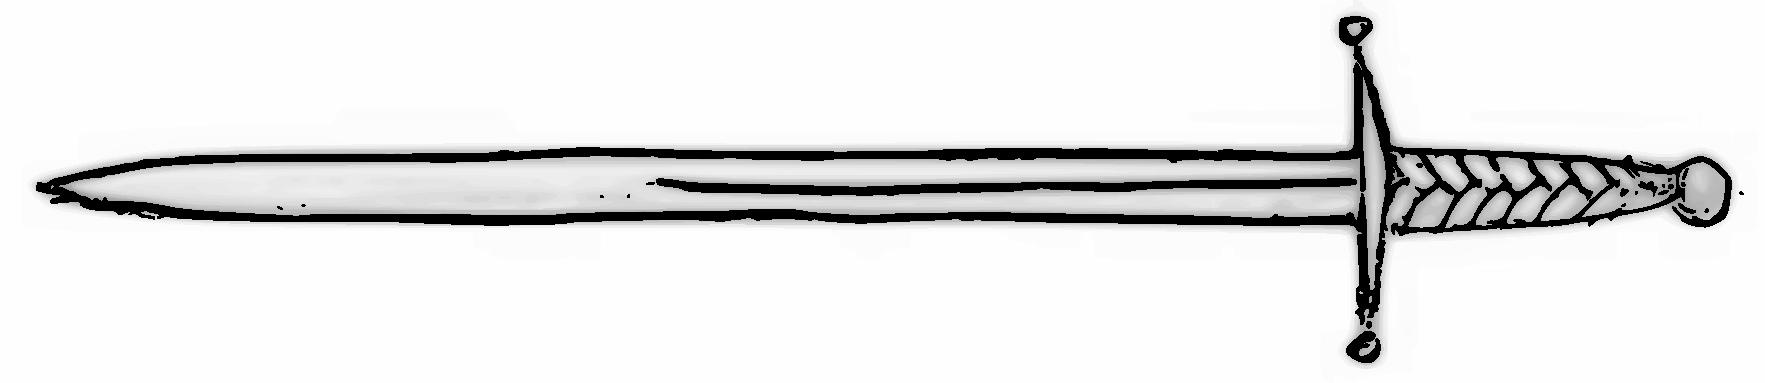
\includegraphics[width=\columnwidth]{bastardsword.pdf}\label{bastardsword}

\index{Swords!Bastard}\paragraph{Sword, Bastard:} Similar to a long sword but with a longer haft.  It can be wielded one-handed or two-handed increasing its damage output.

\columnbreak

\noindent
\begin{minipage}{\columnwidth}

\index{Armor}\captionof{table}{Armor}\label{armor}
\noindent
\begin{tabular}{|p{0.32\columnwidth}|p{0.19\columnwidth}|p{0.17\columnwidth}|p{0.12\columnwidth}|}
\hline
Armor			& Cost	& Wt (lb.)	& AC \\
\hline\hline
\rowcolor[gray]{.9}Banded mail		& 200 gp	& 35	& 4 \\
Brigandine		& 120 gp	& 35	& 6 \\
\rowcolor[gray]{.9}Bronze plate mail	& 400 gp	& 45	& 4 \\
Chain mail		& 75 gp	& 40	& 5 \\
\rowcolor[gray]{.9}Field plate		& 2,000 gp	& 60	& 2 \\
Full plate		& (3d3~+~1) $\times$~1,000 gp	& 70	& 1 \\
\rowcolor[gray]{.9}Leather			& 5 gp	& 15	& 8 \\
Padded			& 4 gp	& 10	& 8 \\
\rowcolor[gray]{.9}Plate mail		& 600 gp	& 50	& 3 \\
Scale mail		& 120 gp	& 40	& 6 \\
\rowcolor[gray]{.9}Splint mail		& 80 gp	& 40	& 4 \\
Studded leather	& 20 gp	& 25	& 7 \\
\hline
\end{tabular}

\end{minipage}

\index{Armor Class!from Armor}\index{Armor}Wearing armor sets a character's base AC to the number listed (the lower the number the better).  If, usually through magic, the character's AC is lower than the listed number (before dexterity is counted), the armor doesn't benefit his AC, but any other benefits and penalties still apply.  The armor names are generic.  Specialized names can be used if the GM prefers.  The armor listed is for man-sized humanoids (including dwarves).

\index{Full Plate}\paragraph{Full Plate:} Gothic-style armor made up of interlocking angled plates and ornamental etchings.  The price varies by manufacturer from 4,000--10,000 gp ((3d3~+~1)~$\times$~1,000 gp).  Each suit must be custom crafted for the wearer.  There's a 20\% chance that a particular suit can be refitted to another wearer.  Because of this, there are few buyers of used full plate except collectors.  A blacksmith may buy a suit to melt the metal down but they'll offer a much-reduced price.

\index{Shields}

\noindent
\begin{minipage}{\columnwidth}

\captionof{table}{Shields}\label{shields}
\noindent
\begin{tabular}{|p{0.18\columnwidth}|p{0.12\columnwidth}|p{0.1\columnwidth}|p{0.14\columnwidth}|p{0.21\columnwidth}|}
\hline
Shield			& Cost	& Wt (lb.)	& \# of Attacks	& AC bonus \\
\hline\hline
\rowcolor[gray]{.9}Body or tower	& 10 gp	& 15	& All + cover		& $-1$/ $-2$ v. missiles \\
Buckler			& 1 gp	& 3		& 1					& $-1$ \\
\rowcolor[gray]{.9}Medium			& 7 gp	& 10	& 3					& $-1$ \\
Small			& 3 gp	& 5		& 2					& $-1$ \\
\hline
\end{tabular}

\end{minipage}

\index{Armor Class!from Shields}\paragraph{Shields:}  Shields provide an AC bonus when certain factors are met.  Shields usually only protect against attacks from the front, however, shields (except bucklers) can be slung across the back to protect against attacks from behind.  Shield size is relative to the character's size; a giant's small shield functions as a medium shield for a human and as a body shield for a halfling.

\index{Bucklers}\paragraph{Buckler:} strapped to the forearm, it allows the wielder to use both hands.  It improves the wielder's armor class by 1 against one frontal attack per round (wielder's choice).  

\index{Small Shields}\paragraph{Small shield:} strapped to the forearm and gripped by the hand, it allows the wielder to hold small items (but not wield weapons) and improves armor class by 1 against two frontal attacks per round (wielder's choice).  

\index{Medium Shields}\paragraph{Medium shield:} functions like the small shield, but its weight restricts the shield hand from doing anything except balance the shield.  A medium shield improves armor class by 1 against any 3 frontal attacks.

\index{Body Shields}\paragraph{Body shield (also called a pavise or tower shield):} functions like the medium shield, improving AC by 1 against any number of frontal melee attacks and by 2 against any number of ranged frontal attacks.

\noindent
\begin{minipage}{\columnwidth}

\captionof{table}{Helmets}\label{helmets}
\noindent
\begin{tabular}{|p{0.18\columnwidth}|p{0.08\columnwidth}|p{0.08\columnwidth}|p{0.26\columnwidth}|p{0.15\columnwidth}|}
\hline
Helmet		& Cost	& Wt (lb.)	& Armor type match												& AC Penalty* \\
\hline\hline
\rowcolor[gray]{.9}Great helm	& 30 gp		& 10	& Heavy armor- banded or better									& +1 \\
Cap			& 4 gp		& 2		& Light armor- padded, leather, brigandine or studded leather	& +1 \\
\rowcolor[gray]{.9}Coif		& 8 gp		& 5		& Medium armor- chain or scale									& +1 \\
Basinet or Closed face	& 20 gp	& 10	& Heavy armor- banded or better							& +1 \\
\rowcolor[gray]{.9}Open face	& 15 gp		& 5		& Medium or heavy- chain or better								& +1 \\
\hline
\end{tabular}
\noindent\begin{tabular}{p{.95\textwidth}}
*Apply this penalty to overall AC if a helmet is not worn, since wearing the helmet is required to gain full protection from the armor. \\
\end{tabular}\vspace{.5em}

\end{minipage}

\index{Helmets}\paragraph{Helmets:} Armor type indicates the armor most commonly associated with the helmet. Technically any helmet can be paired with any armor, but the GM may temporarily impose penalties to the character's charisma score if they are mismatched (it would be like wearing a baseball uniform and a football helmet, or maybe the other way around).  ``Banded or better" includes splint and bronze plate, as well as steel plate armors.  Brief descriptions of the various helmets follow:

\paragraph{Cap:} a padded, leather or steel skullcap.

\paragraph{Coif:} a padded chain mail hood made of steel.

\paragraph{Open-face:} made of reinforced leather, steel or bronze, covers most of the head, except the face and neck.  It commonly includes a nose guard.

\paragraph{Basinet (close-faced):} similar to open-faced, but includes a hinged visor/faceplate.

\paragraph{Great helm:} a massive steel or bronze helmet that covers the entire head, neck, and often the upper shoulders.  It has narrow eye slits and small air holes for breathing.  The visor/faceplate is not removable.  Customized great helms can be quite impressive. 

\index{Armor!for Smaller and Larger Humanoids}\paragraph{Armor for Smaller and Larger Humanoids:} Humanoids exceptionally larger or shorter must be custom fit, which modifies the weight and cost of the armor.  

\noindent
\begin{minipage}{\columnwidth}

\captionof{table}{Armor for Smaller and Larger Humanoids}\label{smallerlarger}
\noindent
\begin{tabular}{|p{0.45\columnwidth}|p{0.17\columnwidth}|p{0.23\columnwidth}|}
\hline
Size of Humanoid		& Cost			& Weight \\
\hline\hline
\rowcolor[gray]{.9}Tiny or Smaller (pixie)	& $\times$$^1$/$_2$	& $\times$$^1$/$_1$$_0$ \\
Small (halfling)		& $\times$1			& $\times$$^1$/$_2$ \\
\rowcolor[gray]{.9}Large (ogre)			& $\times$2--$\times$4		& $\times$1$^1$/$_2$--$\times$2 \\
Huge (giant)			& $\times$4--$\times$8		& $\times$2--$\times$6 \\
\rowcolor[gray]{.9}Gigantic (titan)		& $\times$8--$\times$16	& $\times$6--$\times$12 \\
\hline
\end{tabular}

\end{minipage}

\subsection*{DONNING ARMOR}

\index{Armor!Donning Armor}Donning armor takes time.  Brigandine, leather, padded, and studded leather armor can be donned in one round with assistance.  Banded, chain, scale, and splint mail can be donned in two rounds with assistance.  Without assistance, the time is doubled for all cases.  Bronze plate, field plate, full plate, and plate mail can be donned in 1d6~+~4 rounds with assistance.  Without assistance, the time is tripled for donning plate armor.

Characters can don armor hastily.  Donning non-plate armor hastily takes one round but reduces the AC bonus by 1 (the armor bonus can never be worse than 8).  Hastily donning plate armor improves a character's AC by 1 from base 10 for every round spent dressing.  Removing non-plate armor takes one round and 1d4~+~1 rounds for plate.  Removing plate armors can be done in half the time (round up) by cutting straps, but the armor is thereafter useless until repaired (the cost is up to the GM). 

\section{ENCUMBRANCE}

\subsubsection*{Maximum Encumbrance}

\index{Encumbrance}In simplest terms, all creatures, including the characters, are allowed to carry and wear as much gear as desired without exceeding their strength---max carrying weight score in pounds, up to their maximum carrying capacity.  When both maximum carrying capacity and maximum carrying weight are reached, a character is at his maximum encumbrance. 

\subsubsection*{Maximum Carrying Capacity}

A creature's maximum carrying capacity is limited by its physical size and shape, and is determined solely by the number and size of objects carried or worn, regardless of the object's weight.  Reaching one's maximum carrying capacity may inflict penalties.  However, many of these penalties are obvious and are already built into the rules.  For example, one cannot use a shield or wield a weapon if it's carrying a large bag of coins in each hand or a huge treasure chest requiring both hands.  A creature incurs additional penalties to his attack and AC if it is both carrying its maximum capacity and is more than lightly encumbered (See Below). 

\subsubsection*{Maximum Capacity for Human-shaped Creatures}

To determine when a human-shaped creature (or a biped), including humans, demi-humans, as well as most humanoids and giant-kind, is carrying its maximum carrying capacity, use the following examples.  

In addition to normal clothing and armor (if any):

A small-sized biped can carry up to twenty tiny-sized objects (attached to a belt, cloak liner, or bandoleer), four small-sized objects (two on each hip and two slung around its back), and two medium-sized objects (one in each hand).  A smaller than man-sized backpack and two small belt pouches can also be worn to carry extra miscellaneous gear.  

A man-sized biped can carry up to twenty small-sized objects (attached to a belt, cloak liner, or bandoleer), four medium-sized objects (two on each hip and two slung around its back), and two large-sized objects (one in each hand).  A man-sized backpack and two large belt pouches can also be worn.  

A large-sized biped can carry up to twenty medium-sized objects (attached to a belt, cloak liner, or bandoleer), four large-sized objects (two on each hip and two slung around its back), and two huge-sized objects (one in each hand).  A larger than man-sized backpack and two huge belt pouches can also be worn.  

Tiny-sized creatures carry small, tiny and even smaller objects, while huge-sized and larger bipeds can carry ever-larger objects before reaching their maximum carrying capacity.  In addition, two objects of the same size may be exchanged for one object of the next larger size, or vice versa, (within reason) in this way a large number of combinations of gear and equipment are possible even for the smallest character.

Due to these restrictions, a creature may be carrying its maximum capacity before reaching its maximum weight score.  An empty huge-sized treasure chest does not weigh very much but does count as 2 large, 4 medium or 8 small objects toward the creature's maximum carrying capacity.  

Likewise, a creature may be carrying its maximum weight allowed and not yet be at its maximum capacity, as when a character carries a huge chest with nearly all of his other gear and heavy gold treasure inside of it.  A fighter with a low strength score but wearing heavy plate armor, great helm, shield and a two-handed sword, etc. could be overwhelmingly encumbered by the weight of the objects.  In this case, he would suffer movement penalties, but not penalties to his attacks or AC because he has not reached his maximum carrying capacity.

\subsubsection*{Encumbrance for Man-sized Bipeds}

Encumbrance represents the penalties that a creature suffers, associated with number of pounds that it carries and/or wears.  There are seven stages of encumbrance in increasing order of discomfort: non-encumbered, lightly encumbered, moderately, heavily, severely, and overwhelmingly encumbered.  

To determine encumbrance, add together the weight of all of the character's carried or worn possessions (including about 5 lbs. for man-sized clothing).  If the total is less than or equal to the non-encumbrance score, the character suffers no penalties.  If the weight exceeds the non-encumbrance score consult the table below.  

The row across the top reflects the stage of encumbrance the creature suffers if it is at full carrying capacity.  The rows across the bottom determine the creature's modified movement values due to its encumbrance.  The first of these is for bipeds with a normal movement value of 12 (elves, humans, half-elves).  The second row is for bipeds with a normal movement value of 9 (dwarves), and the third is for bipeds with a normal movement value of 6 (gnomes and halflings).

 
\subsubsection*{Effects of Encumbrance}

\index{Armor Class!Effects of Encumbrance}The character's current encumbrance may negatively affect their ability to move and to defend themselves if they are also at their maximum capacity.

\paragraph{Non-Encumbered:} This value is found on the main strength table.  A creature suffers no penalties to movement, AC or attacks, as long as the weight of his gear is equal to or less than this score.

\paragraph{Lightly Encumbered:} This stage of encumbrance, starting at 0.01 pound above the creature's strength---non-encumbered score, indicates only mild movement value penalties.  

\paragraph{Moderately Encumbered:} This stage of encumbrance, starting at 0.01 pound above the creature's highest light encumbrance score, indicates moderate movement value penalties, and if the creature is carrying its maximum capacity, it also suffers a $-1$ penalty to attacks.

\paragraph{Heavily Encumbered:} This stage of encumbrance, starting at 0.01 pound above the creature's highest moderate encumbrance score, indicates significant movement value penalties, and if the creature is carrying its maximum capacity, it also suffers a $-2$ penalty to attacks and +1 penalty to its AC.

\paragraph{Severely Encumbered:} This stage of encumbrance, starting at 0.01 pound above the creature's highest heavy encumbrance score, indicates severe movement value penalties, and if the creature is carrying its maximum capacity, it also suffers a $-4$ penalty to attacks, and a +3 penalty to its AC.

\paragraph{Overwhelmingly Encumbered:} The maximum stage of encumbrance, starting at 0.01 pound above the creature's highest severe encumbrance score and topping out at a character's maximum carry weight as found on the main strength table. This indicates a movement value of only 1, and if the creature is carrying its maximum capacity, it also suffers a $-4$ penalty to attacks, and a +3 penalty to its AC.

\end{multicols}

\noindent
\begin{minipage}{\columnwidth}

\captionof{table}{Encumbrance for Man-sized Bipeds}\label{encbipeds}
\noindent
\begin{tabular}{|p{0.080\textwidth}|p{0.066\textwidth}|p{0.066\textwidth}|p{0.066\textwidth}|p{0.066\textwidth}|p{0.066\textwidth}|p{0.066\textwidth}|p{0.066\textwidth}|p{0.066\textwidth}|p{0.066\textwidth}|p{0.066\textwidth}|}
\hline
 & \multicolumn{10}{c|}{Encumbrance in Pounds} \\
Str	& \multicolumn{3}{c|}{Lightly}	& \multicolumn{3}{c|}{Moderately}	& \multicolumn{3}{c|}{Heavily}	& Sev \\
\hline\hline
\rowcolor[gray]{.9}1		& $^1$/$_2$ 	& $^3$/$_4$		& 1		& 1$^1$/$_4$ 	& 1$^1$/$_2$ 	& 1$^3$/$_4$	& 2		& 2$^1$/$_4$ 	& 2$^1$/$_2$  	& 2$^3$/$_4$  \\
2		& 1$^1$/$_2$ 	& 2		& 2$^1$/$_4$ 	& 2$^3$/$_4$ 	& 3		& 3$^1$/$_4$ 	& 3$^3$/$_4$ 	& 4		& 4$^1$/$_4$  	& 4$^3$/$_4$  \\
\rowcolor[gray]{.9}3		& 5$^1$/$_2$ 	& 6		& 6$^1$/$_2$ 	& 7		& 7$^1$/$_2$ 	& 8		& 8$^1$/$_2$ 	& 9		& 9$^1$/$_4$		& 9$^3$/$_4$  \\
4--5		& 11	& 12	& 13	& 14	& 15	& 16	& 17	& 18	& 19	& 19$^1$/$_2$  \\
\rowcolor[gray]{.9}6--7		& 23	& 26	& 29	& 32	& 35	& 38	& 41	& 44	& 47	& 50 \\
8--9		& 40	& 45	& 50	& 55	& 60	& 65	& 60	& 75	& 80	& 85 \\
\rowcolor[gray]{.9}10-11	& 46	& 52	& 58	& 64	& 70	& 76	& 82	& 88	& 94	& 100 \\
12--13	& 53	& 61	& 69	& 77	& 85	& 93	& 101	& 109	& 117	& 125 \\
\rowcolor[gray]{.9}14--15	& 65	& 75	& 85	& 95	& 105	& 115	& 125	& 135	& 145	& 155 \\
16		& 80	& 90	& 100	& 110	& 120	& 130	& 140	& 150	& 160	& 170 \\
\rowcolor[gray]{.9}17		& 97	& 109	& 121	& 133	& 145	& 157	& 169	& 181	& 193	& 210 \\
18		& 123	& 136	& 149	& 162	& 175	& 188	& 201	& 214	& 227	& 245 \\
\rowcolor[gray]{.9}18/50	& 148	& 161	& 174	& 187	& 200	& 213	& 226	& 239	& 252	& 270 \\
18/75	& 173	& 186	& 199	& 212	& 225	& 238	& 251	& 264	& 277	& 295 \\
\rowcolor[gray]{.9}18/90	& 198	& 211	& 224	& 237	& 250	& 263	& 276	& 289	& 302	& 320 \\
18/99	& 248	& 261	& 274	& 287	& 300	& 313	& 326	& 339	& 352	& 365 \\
\rowcolor[gray]{.9}18/00	& 348	& 361	& 374	& 387	& 400	& 413	& 426	& 439	& 452	& 470 \\
19		& 498	& 511	& 523	& 536	& 549	& 562	& 575	& 588	& 611	& 625 \\
\rowcolor[gray]{.9}20		& 540	& 555	& 570	& 585	& 600	& 615	& 630	& 645	& 670	& 685 \\
21		& 650	& 665	& 680	& 695	& 710	& 725	& 745	& 765	& 780	& 795 \\
\rowcolor[gray]{.9}22		& 802	& 819	& 836	& 853	& 870	& 887	& 904	& 921	& 937	& 954 \\
23		& 952	& 969	& 986	& 1,000	& 1,017	& 1,035	& 1,052	& 1,069	& 1,086	& 1,110 \\
\rowcolor[gray]{.9}24		& 1,255	& 1,275	& 1,295	& 1,315	& 1,335	& 1,355	& 1,375	& 1,395	& 1,415	& 1,430 \\
25		& 1,545	& 1,565	& 1,585	& 1,605	& 1,625	& 1,645	& 1,665	& 1,685	& 1,705	& 1,730 \\
\hline\hline
\rowcolor[gray]{.9}MV 12	& 11	& 10	& 9		& 8		& 7		& 6		& 5		& 4		& 3		& 2 \\
MV 9	& 8	 	& 8		& 7		& 6		& 5		& 5		& 4 	& 3		& 2		& 2 \\
\rowcolor[gray]{.9}MV 6	& 5	 	& 5		& 4		& 4		& 3		& 3		& 2		& 2		& 1		& 1 \\
\hline
\end{tabular}

\end{minipage}

\begin{multicols}{2}

\noindent
\includegraphics[width=\columnwidth, height=2in]{testblock.pdf}

\subsubsection*{Encumbrance for Larger and Smaller Bipeds}

Small-sized and smaller creatures can carry less weight than their man-sized counterparts.  For tiny-sized creatures multiply all values by 0.50, and for small-sized creatures multiply all values by 0.75.  

Large-sized and larger creatures can carry more weight than their man-sized counterparts.  For large-sized creatures multiply all values by 2, for huge-sized creatures multiply by 4, and for gigantic-sized creatures multiply all values by 8.  
 
\subsubsection*{Encumbrance for Quadrupeds}

Creatures with four or more legs can also carry more weight than their strength would indicate.  For tiny-sized quadrupeds multiply all values by 0.75, small-sized quadrupeds use the values unchanged, for man-sized quadrupeds multiply all values by 1.5, for large-sized quadrupeds multiply all values by 3, for huge-sized quadrupeds multiply by 6, and for gigantic-sized quadrupeds multiply all values by 12.  

\subsubsection*{Encumbrance for Domestic Animals}

\index{Animals!Encumbrance}A pack animal or mount suffers from encumbrance differently than other creatures.  A mount can be non-encumbered if its total weight, including a rider, is equal to or less than the value shown below, but is either lightly encumbered or heavily encumbered, otherwise.  Movement modifiers and combat penalties are shown at the bottom of the table.  An animal collapses if its heaviest encumbrance value in pounds is exceeded whether carrying a rider or being used as a pack animal.  Whenever a mount carries a man-sized rider and whenever any animal is heavily encumbered, it is always considered to be at its maximum carrying capacity (even though more weight can be added).  While at maximum capacity an animal suffers reduced movement value, and penalties to its attacks and AC, as appropriate.  A lightly encumbered mount without a rider or a lightly encumbered pack animal does not suffer penalties to its attacks or AC, but still suffers the movement penalty.  

The weight a flying mount may carry and still fly may be listed in its description.  If undetermined, assume the average flying mount cannot fly if lightly encumbered or more.

\noindent
\begin{minipage}{\columnwidth}

\captionof{table}{Encumbrance for Domestic Animals}\label{encdomestic}
\noindent
\begin{tabular}{|p{0.19\columnwidth}|p{0.13\columnwidth}|p{0.23\columnwidth}|p{0.25\columnwidth}|}
\hline
	& \multicolumn{3}{c|}{Encumbrance in Pounds} \\
Common Animal	& Non-Enc	& Light	& Heavy \\
\hline\hline
\rowcolor[gray]{.9}Camel			& 330	& 500	& 660 \\
Hunting dog		& 15	& 20	& 30 \\
\rowcolor[gray]{.9}Elephant		& 500	& 750	& 1,000 \\
Horse, draft	& 260	& 390	& 520 \\
\rowcolor[gray]{.9}Horse, heavy	& 260	& 390	& 520 \\
Horse, light	& 170	& 255	& 340 \\
\rowcolor[gray]{.9}Horse, medium	& 220	& 330	& 440 \\
Horse, riding	& 180	& 270	& 360 \\
\rowcolor[gray]{.9}Mule			& 250	& 375	& 50 \\
Ox				& 220	& 330	& 440 \\
\rowcolor[gray]{.9}Yak				& 220	& 330	& 440 \\
\hline\hline
MV	& Normal	& MV $\times$$^2$/$_3$	& MV $\times$$^1$/$_3$ \\
\rowcolor[gray]{.9}Penalties	& None	& $-1$ THACO	& $-2$ THACO/ +1 AC \\
\hline
\end{tabular}

\end{minipage}

\section{EXAMPLE: CREATING A CHARACTER}

Justin, a player, and Tommy, his GM, both sit down to create a new character.  Tommy wants Justin to roll using the traditional method (3d6 for each score).  He comes up with the following scores:

Strength 15

Dexterity 12

Constitution 14

Intelligence 12

Wisdom 11

Charisma 10

The character has above average strength and constitution and would make a good fighter.  Justin decides he wants to be a dwarf, improving his character's constitution by 1 point and reducing his charisma by 1 point.  As a fighter, Justin rolls his d10 hit die and rolls a 2, a poor number.  Tommy allows him to re-roll his hit die but says the re-roll must be taken even if it's lower.  Justin rolls an 8 and adds +1 for his constitution for 9 HP total.  Justin's fighter has 4 combat skill points as a 1\textsuperscript{st} level fighter and exchanges 2 points to gain the axe weaponry group (including battle axes, hand/throwing axes, and pole axes).  He then chooses to exchange one CSP to gain specialization with battle axe, and his last CSP is exchanged for the weapon-shield combat method.

Justin rolls 11 for his fighter's starting currency, giving him 110 gp total.  Justin buys a battle axe, five hand axes, chain mail, a medium shield, and some provisions.  His character is finished and Justin adds some final cosmetic touches; platinum blonde hair, piercing blue eyes, a distinctive scar along the left cheek, and a grating voice.  Justin names his dwarf fighter Tharn Bittermead and writes up a paragraph long back-story to supply Tommy with an idea of how the character fits into his world.  Tharn's final character sheet would look something like this:

\paragraph{Tharn Bittermead,} Dwarven Fighter 1

\noindent MV 6

\noindent HP 9

\noindent Strength 15

\noindent Dexterity 12

\noindent Constitution 15

\noindent Intelligence 12

\noindent Wisdom 11

\noindent Charisma 9

\columnbreak

\noindent THACO 20 (+1 to attack, battle axes)

\noindent AC 4 (Chain mail~+~medium shield)

\noindent Battle Axe (Specialization) M/L 1d8~+~2/1d8~+~2

\noindent Hand Axe (Skilled) M/L 1d6~+~2/1d4~+~2

\noindent Weapon-shield method (Skilled)

\noindent Backpack

\noindent \hspace{2em}Rations (5)

\noindent \hspace{2em}Hooded lantern

\noindent \hspace{2em}Oil (3)

\noindent \hspace{2em}Flint and steel

\vspace{1em}

Justin would probably also add notes about his racial abilities, modifiers granted by his ability scores and combat skills as well as his THACO and saving throws so he won't have to look them up every time.

\noindent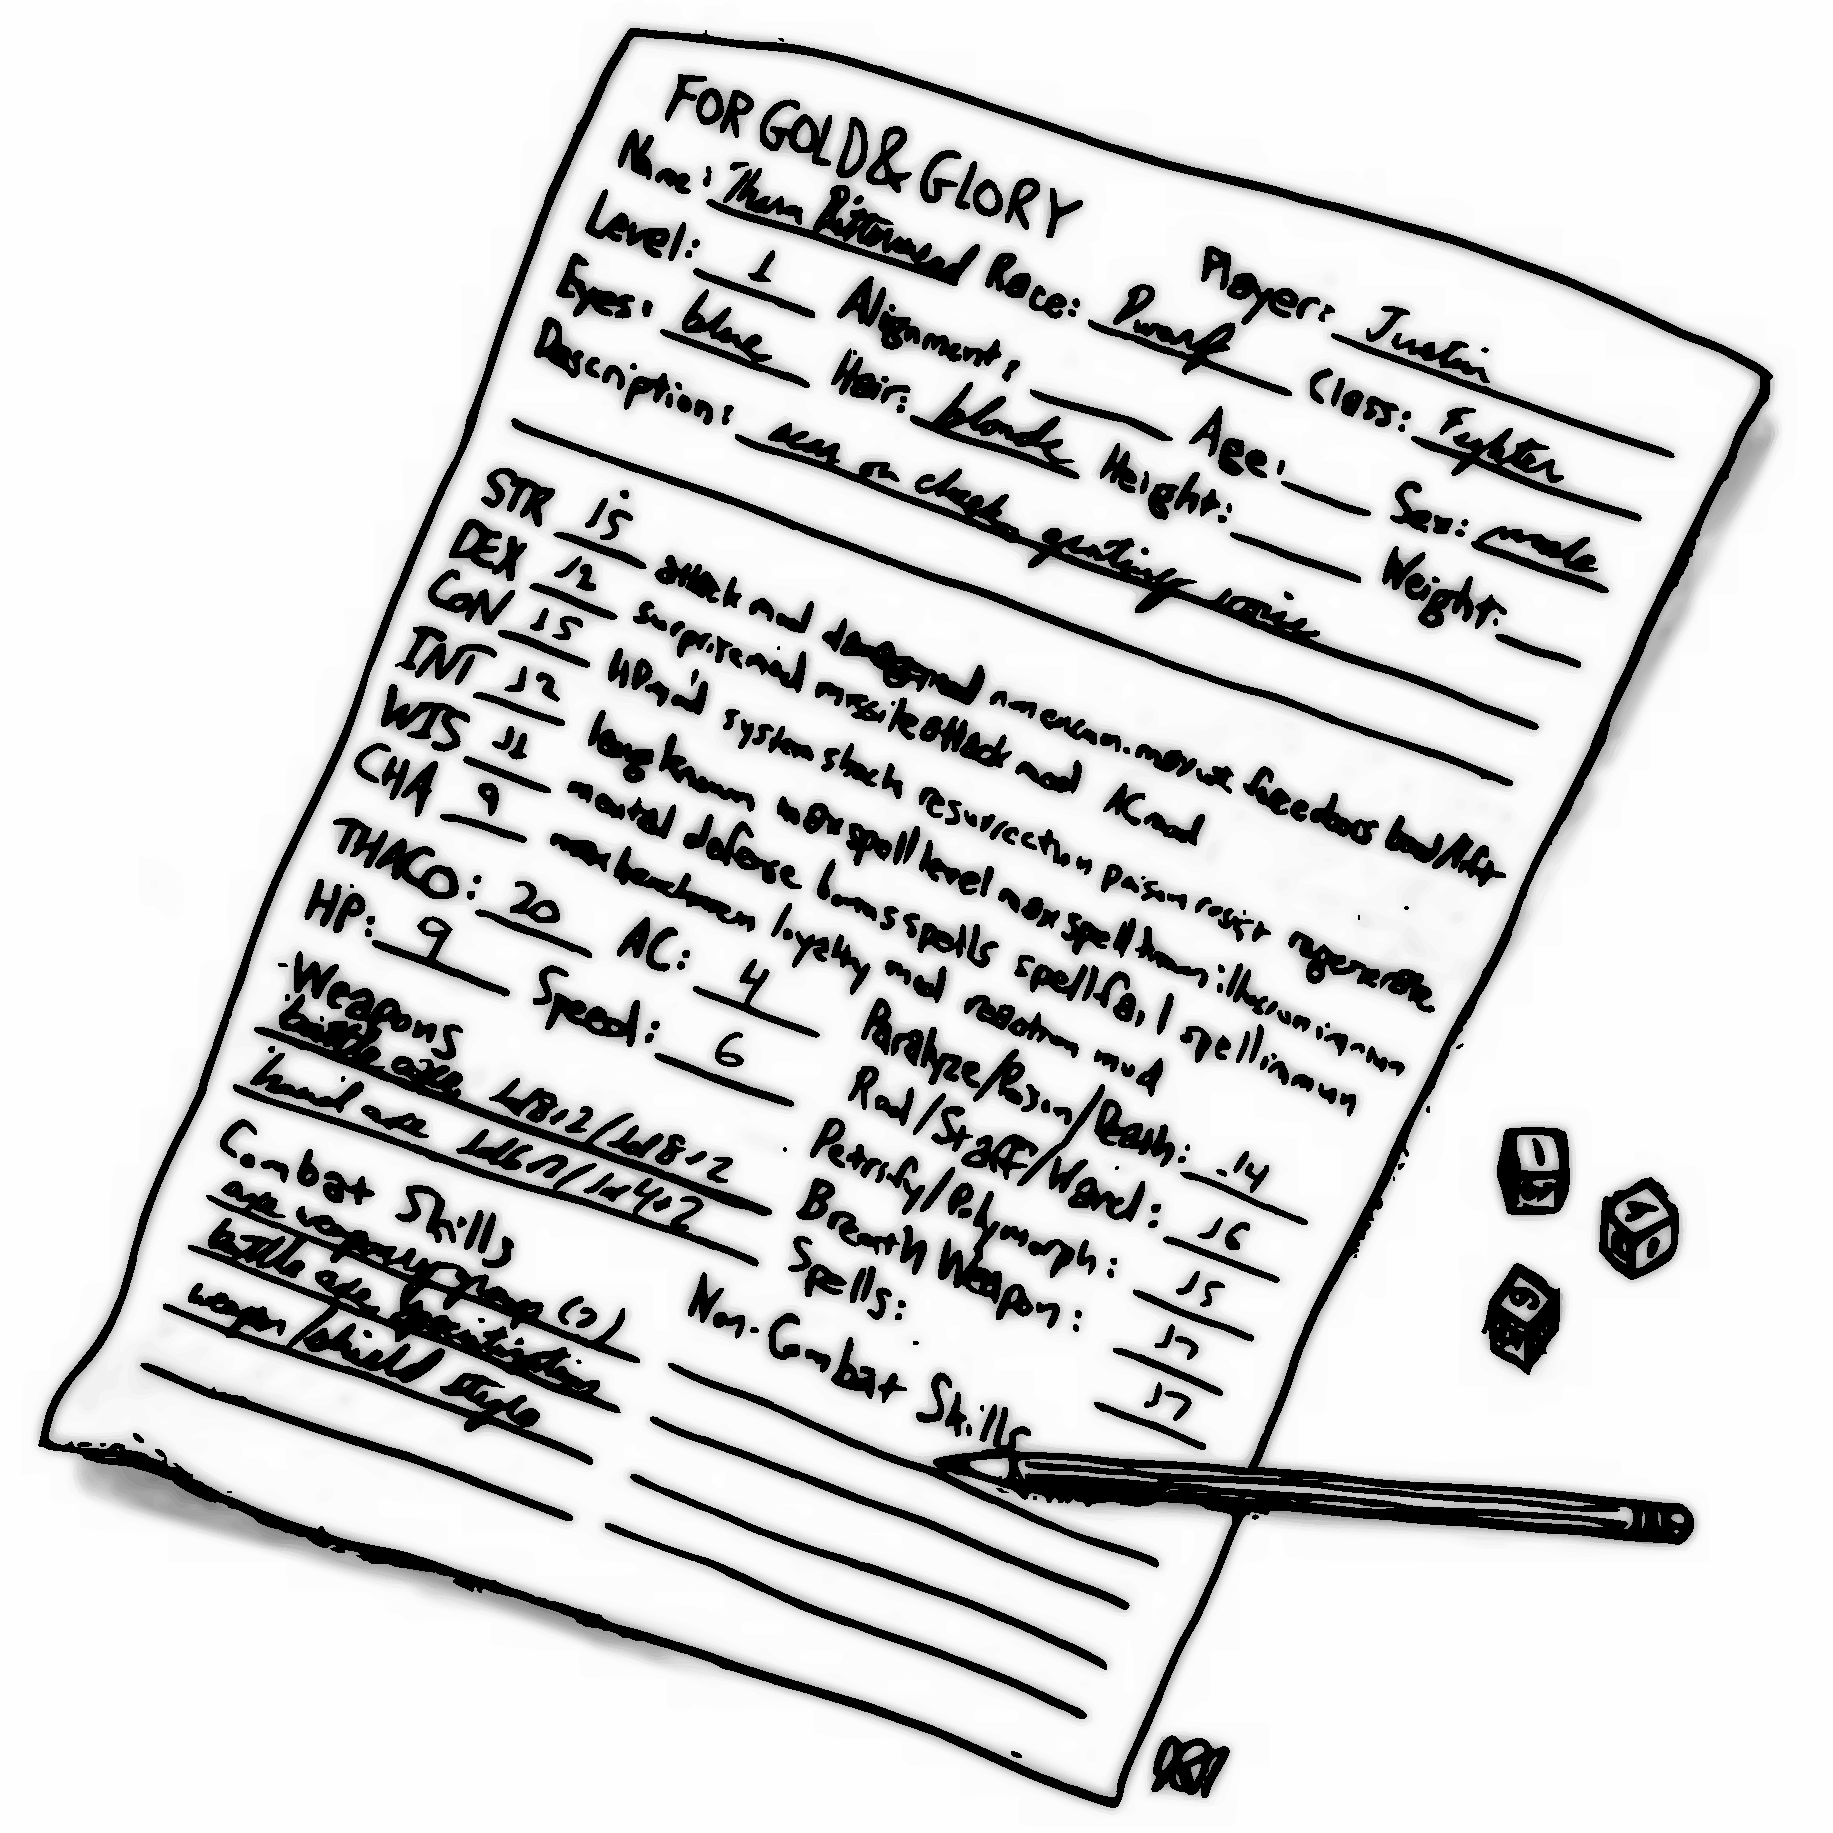
\includegraphics[width=\columnwidth]{bittermead.pdf}\label{bittermead}


\end{multicols}
